\documentclass[a4paper,12pt]{report}

\usepackage{alltt, fancyvrb, url}
\usepackage{graphicx}
\usepackage[utf8]{inputenc}
\usepackage{float}
\usepackage{xcolor}
\usepackage{hyperref}

% Questo commentalo se vuoi scrivere in inglese.
\usepackage[italian]{babel}

\usepackage[italian]{cleveref}

\begin{document}

\title{RelazioneOOP - ArtRat}

\begin{figure}
    \centering
    
\includegraphics[width=0.5\linewidth]{logo.png}
    \label{fig:enter-label}
\end{figure}

\author{Matteo Tonelli, Samuele Trapani, Cristian Di Donato, Manuel Benagli}
\date{December 2024}

\maketitle

\newpage

\newpage
\tableofcontents
\clearpage

\chapter{Analisi}
\section{Descrizione e Requisiti}
ArtRat vuole essere un gioco di azione stealth , ispirato al gioco già esistente "Robbery Bob", in cui il giocatore veste i panni di un ladro d'appartamento appassionato di quadri.
Il gioco si svolge all'interno di un hotel in cui il ladro, chiamato LuPino, si intrufola all'interno delle camere per collezionare più quadri possibili senza essere scoperto.
Il ladro potrà essere fermato da:
\begin{itemize}
    \item Allarme : una volta entrato nella camera, vi sarà un'allarme che dopo due minuti farà arrivare la polizia sul posto e dunque rendendo impossibile a LuPino la riuscita del furto.
    \item Personale : vi sarà in ogni camera il personale di guardia, incaricato di sorvegliare i quadri, che una volta visto LuPino, cercherà di catturarlo.
\end{itemize}
Più il giocatore sarà abile e veloce a collezionare quadri, più punti gli verranno assegnati una volta uscito dalla camera (simulando dunque la vendita del bottino). 
Al ladro sarà anche disponibile un negozio per spendere i "punti" guadagnati dopo ogni furto comprando powerup e consumabili per rendere più facile il furto, o semplicemente per variare lo stile di gioco:
\begin{itemize}
    \item PowerUp : modificatori permanenti delle abilità del ladro, ad esempio un aumento della velocità
    \item Consumabili : effetti simili ai PowerUp ma ad utilizzo singolo per furto, ad esempio attivando un consumabile il ladro potrebbe guadagnare il doppio rispetto al solito esclusivamente dal suo prossimo furto.
\end{itemize}

\subsubsection{Requisiti funzionali}
\begin{itemize}
    \item La generazione delle stanze in ogni appartamento dovrà essere casuale
    \item I nemici dovranno essere capaci di individuare il giocatore e di rendergli difficile il compito di rubare.
    \item Il timer, rappresentante l'allarme, si attiverà una volta entrato in un appartamento e dovrà scorrere fino all'uscita del giocatore
    \item Il furto dovrà essere comunque possibile nonostante gli impedimenti
    \item Il ladro potrà muoversi in verticale e in orizzontale all'interno del piano potendo anche interagire con gli oggetti presenti nella stanza, ad esempio nascondendosi dietro mobili o rubando quadri
    \item Gli oggetti di interesse garantiranno un guadagno in punti in base alla rarità dell'oggetto
    \item Il negozio in gioco dovrà essere accessibile tra un furto e l'altro e permettere l'acquisto di nuovi power-up e consumabili con i punti guadagnati
\end{itemize}

\subsubsection{Requisiti non funzionali}
\begin{itemize}
    \item Il gioco dovrà essere ottimizzato per avere un gameplay fluido senza eccessivi cali di frame.
    \item ArtRat dovrà avere una grafica minimale in grado di rappresentare gli elementi principali e di far capire al giocatore le azioni disponibili
    \item La finestra di gioco dovrà garantire scalabilità, mantenendo comunque proporzioni adatte.
\end{itemize}

\clearpage
\section{Modello }
In ArtRat, il giocatore si dovrà muovere all'interno di un hotel diviso in appartamenti. Ognuno dei quali è dotato di un allarme centrale che si attiva quando LuPino ne resta all'interno per un certo tempo limite, e di un sistema di stanze ognuna con una disposizione precisa di oggetti e ostacoli.
La stanza dunque è il cuore del gameplay, ogni stanza potrà includere Oggetti D'Interesse che appunto saranno l'obbiettivo principale di LuPino, ma anche ostacoli d'ambiente che costituiranno il "labirinto" in cui il ladro si aggirerà.
Ogni stanza può essere sorvegliata inoltre da una o più guardie che pattugliano la zona; le guardie rappresentano un ostacolo dinamico, obbligando il giocatore a usare le proprie abilità per evitarle.
Il giocatore una volta uscito dall'appartamento avrà accesso al negozio di gioco, in cui potrà spendere i punti guadagnati per comprare oggetti utili al suo compito che porterà con sé nel suo inventario, divisi tra PowerUp e Consumabili che, come spiegato precedentemente, hanno utilizzo diverso.

\begin{figure}[H] % Use [H] to force the placement of the figure
    \centering
    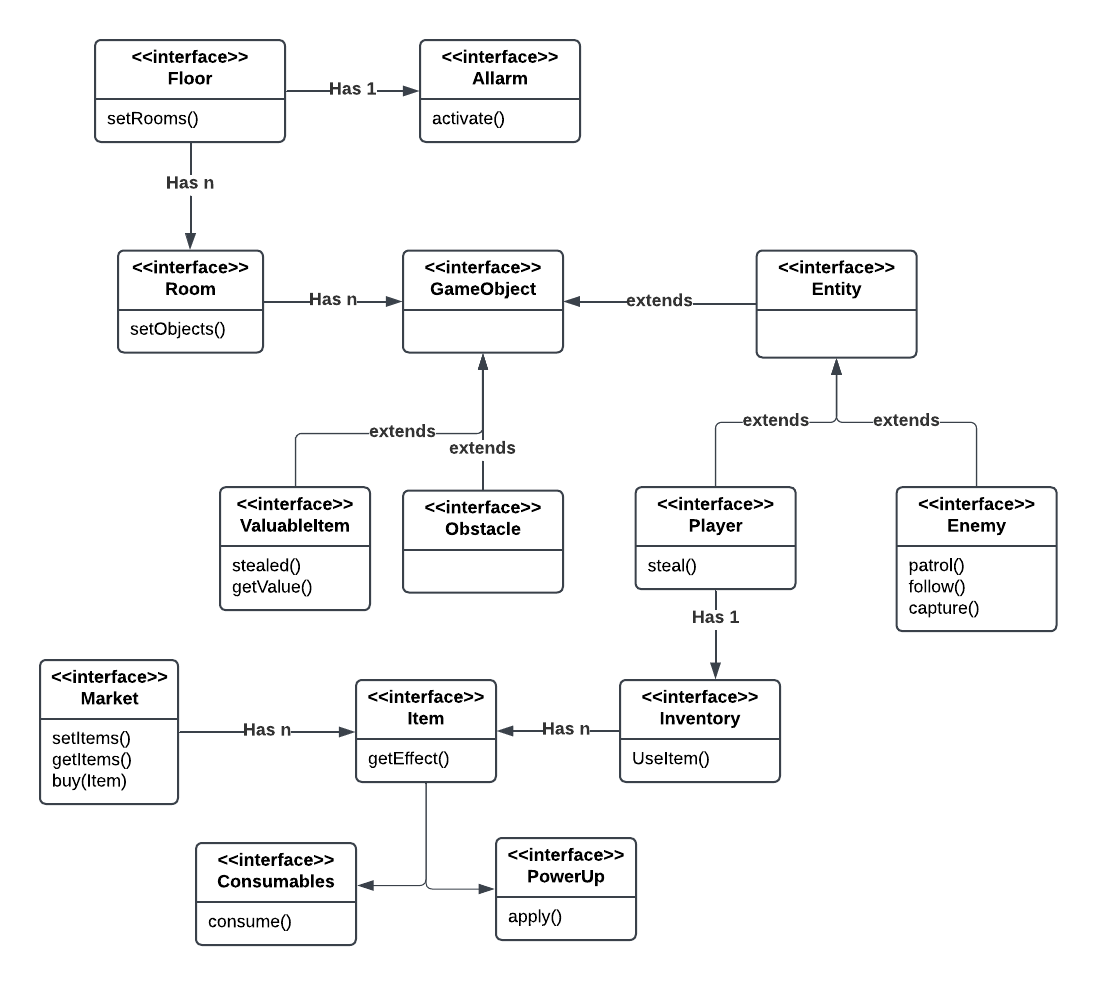
\includegraphics[width=0.9\linewidth]{UML domain model.png}
    \caption{UML domain model}
    \label{fig:enter-label}
\end{figure}

\clearpage

\chapter{Second Section}
This second section\index{section} may include some special 
word, and expand the ones already used\index{keywords!used}.

\end{document}
